\documentclass{article}

\usepackage[utf8]{inputenc}
\usepackage[T1]{fontenc}% optional T1 font encoding
\usepackage[%
    colorlinks=true,
    pdfborder={0 0 0},
    linkcolor=red
]{hyperref}
\usepackage[all]{hypcap}
\usepackage{amsmath}
\interdisplaylinepenalty=2500
\usepackage{graphicx}
\usepackage[cmintegrals]{newtxmath}
\usepackage{cite}
\usepackage{listings}
\usepackage{hyperref}
\usepackage{indentfirst}

\begin{document}

\title{MC 613 - Diagrama de Blocos}
\author{Luiz Eduardo T. C. Cartolano(RA 183012)
        e Yago de Lima Barbosa(RA 188727) }
\date{Junho 2018}

\maketitle

\section{Descrição do projeto}
Na implementação do projeto, seguiremos o seguinte esquema: o jogador utiliza o mouse para marcar sua opção no monitor. O jogo deve permitir escolher qual jogador começa e jogar contra outro ser humano em turnos ou contra uma IA, que obrigatoriamente deve ganhar sempre que possível (o jogo da velha é determinístico). Ao terminar o jogo, mostramos no monitor quem foi o vencedor (ou o empate caso não tenha um) e forneceremos a opção de se iniciar um novo jogo. 

As regras do jogo são bem simples \cite{ref:velha-regras}, basicamente, os jogadores jogam alternadamente, o objectivo é conseguir três círculos ou três xis em linha, quer horizontal, vertical ou diagonal.


\section{Diagrama de Blocos}
O diagrama de blocos para o projeto do Jogo da velha que será implementado pode ser visto na Figura \ref{fig:diagrama}, ele foi criado usando uma ferramenta para desenhos de diagramas do Google e pode ser acessado clicando \href{https://drive.google.com/file/d/1U_X492n2xRLVOVa0kffrWD5SYa2kWRCx/view?usp=sharing}{aqui}. Nele as setas representam dados e os conectores sinais de controles. Uma descrição mais detalhada de cada um dos blocos é dada a seguir.
   
    \subsection{Bloco Mouse}
        \begin{itemize}
            \item \textbf{Entradas:} Dados recebidos na entrada PS2 da placa(de I/O). Posição x e y do mouse advindos de \emph{Atualiza Posição}, com relação a origem adotada no mapeamento de pixels do monitor. E também um sinal do bloco \emph{Valida Clique} informando se o clique recebido foi válido. 
            \item \textbf{Saída:} Posição atual do mouse (para Monitor), dados iniciais da partida (para UC) e jogada do turno(para UC).
            \item \textbf{Função:} Gerenciar as ações a serem tomadas pelo clique do mouse, além de gerenciar o funcionamento dos blocos \emph{Valida Clique e Atualiza Posição} para coletar e processar os dados do mouse.
        \end{itemize}
    
    \subsection{Bloco Valida Clique}
        \begin{itemize}
            \item \textbf{Entradas:} Posições x e y do mouse, recebidas do \emph{Mouse}.
            \item \textbf{Saída:} Um comando informando qual região da tela foi clicada, ou um comando informando que não houve clique em uma região válida.
            \item \textbf{Função:} Gerenciar as ações a serem tomadas pelo clique do mouse, o bloco é responsável por verificar se a região selecionada pelo usuário poderia sofrer tal ação.
        \end{itemize}
        
    \subsection{Bloco Atualiza Posição}
        \begin{itemize}
            \item \textbf{Entradas:} Sinal do \emph{Mouse} com os dados recebidos na entrada PS2.
            \item \textbf{Saída:} Posição atual do mouse, nos eixos x e y, com relação a posição (0,0) do sistema. 
            \item \textbf{Função:} Recebe os dados da entrada PS2 e converte os mesmos em posições (x,y) que serão usadas pelas demais entidades.   
        \end{itemize}
    
    \subsection{Bloco Monitor}
        \begin{itemize}
            \item \textbf{Entradas:} Posição do mouse, oriundos do \emph{Mouse}, e situação atual do jogo, informada pela \emph{UC}.
            \item \textbf{Saída:} Imagem atualizada do jogo (pintura dos pixels) para a porta VGA da placa(I/O).
            \item \textbf{Função:} Manter a tela do jogo atualizada no monitor VGA.
        \end{itemize}

    \subsection{Bloco IA - Inteligência Artificial}
        \begin{itemize}
            \item \textbf{Entradas:} Situação do grid do jogo e um sinal informando que é a sua vez de jogar, ambos informados pela \emph{UC}.
            \item \textbf{Saída:} Melhor jogada para a situação atual do jogo (para a \emph{UC}).
            \item \textbf{Função:} Verificar a melhor jogada possível, de forma a ganhar o jogo sempre que possível ou, no pior dos casos, empatar com o adversário.
        \end{itemize}

    \subsection{Bloco UC - Unidade de Controle}
        \begin{itemize}
            \item \textbf{Entradas:} O \emph{Mouse} informa a \emph{UC} informações básicas do jogo e os comandos realizados pelo usuário. Enquanto a \emph{IA} informa para a \emph{UC} a jogada que ela deseja realizar
            \item \textbf{Saída:} A \emph{UC} envia para o monitor a situação atual do grid do jogo, que deverá ser mostrada no VGA. Enquanto que para a \emph{IA}, ela informa a situação atual do grid do jogo e o momento de jogar.
            \item \textbf{Função:} Controlar o fluxo de dados do projeto, acionar a atualização da tela (feita pelo \emph{Monitor}), acionar a jogada da IA.
        \end{itemize}

\begin{figure}[h!]
    \centering
    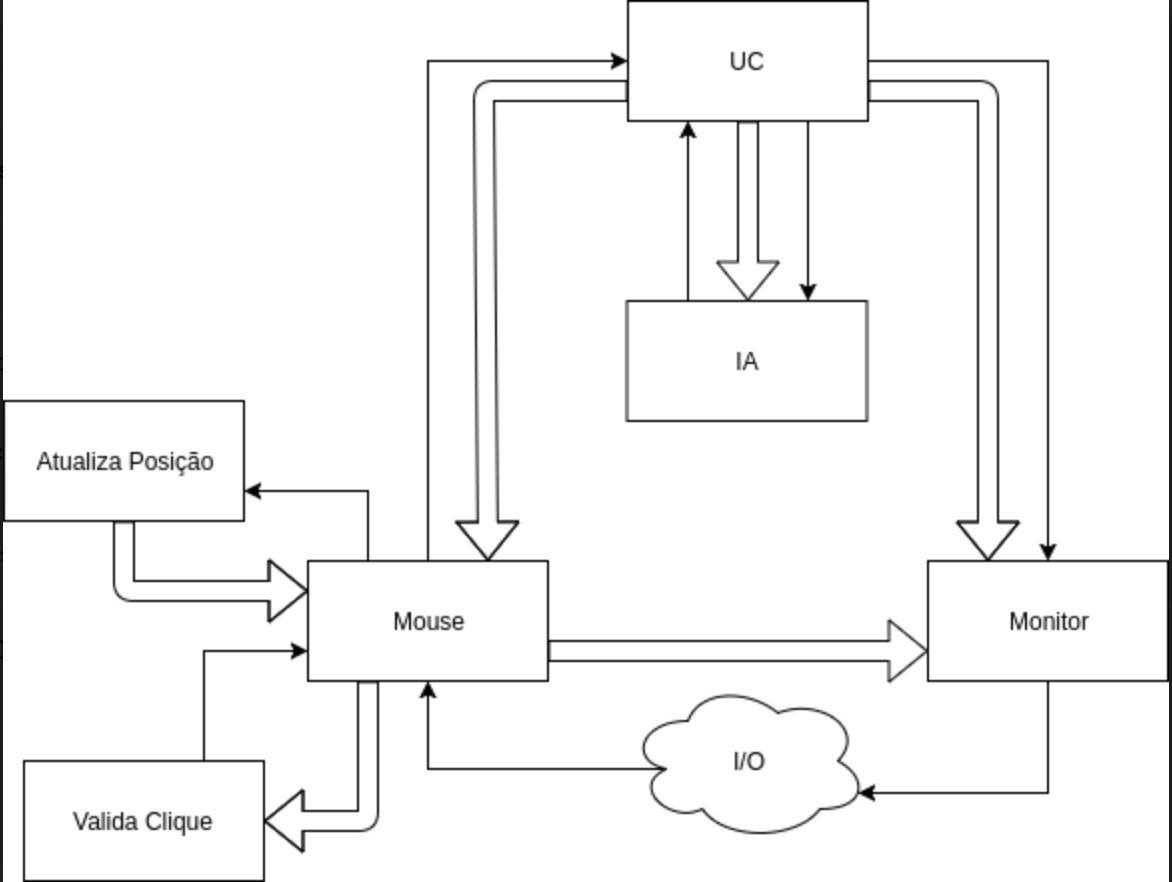
\includegraphics[scale=0.7]{diagrama.png}
    \caption{\label{fig:diagrama}Diagrama de blocos para o projeto de Jogo da Velha da disciplina de MC613.}
\end{figure}


\nocite{*}
\bibliographystyle{plain}
\bibliography{references}

\end{document}
